\section{Normalteiler und Quotientengruppen}

Sei $G$ eine Gruppe.

\begin{definition}[normal, Normalteiler]
	Eine Untergruppe $H\le G$ ist \begriff{normal} (in Zeichen $H\unlhd G$), wenn $g^{-1}hg\in H$ für alle $h\in H$ und $g\in G$. Ein \begriff{Normalteiler} von $G$ ist eine normale Untergruppe von $G$.
\end{definition}

\begin{example}
	\begin{enumerate}[label=(\alph*)]
		\item Ist $G$ abelsch, so ist jede Untergruppe von $G$ ein Normalteiler.
		\item Ist $\phi: G\to H$ ein Gruppenhomomorphismus, so ist $\Ker(\phi)\unlhd G$, denn $\phi(h)=1\Rightarrow\phi(g^{-1}hg)=\phi(g)^{-1}\phi(h)\phi(g)=1$ $\forall g\in G$.
		\item Jede Gruppe $G$ hat die trivialen Normalteiler $1\unlhd G$ und $G\unlhd G$.
	\end{enumerate}
\end{example}

\begin{lemma}
	\proplbl{1_3_3}
	Sei $H\le G$ und $N\unlhd G$.
	\begin{enumerate}[label=(\alph*)]
		\item $H\unlhd G\Leftrightarrow gH=Hg$ für alle $g\in G$
		\item $HN=NH$, $HN\le G$, $N\unlhd HN$, $H\cap N\le N$, $H\cap N\unlhd H$
		\item Sind $N,H\unlhd G$, so ist $H\cap N\unlhd G$, $HN\unlhd G$
		\item Für $g,g'\in G$ ist $gN\cdot g'N=gg'N$
	\end{enumerate}
\end{lemma}
\begin{proof}
	\begin{enumerate}[label=(\alph*)]
		\item Hinrichtung: $\forall g\in G$, $\forall h\in H$: $g^{-1}hg\in H\Rightarrow gHg^{-1}\subseteq H\Rightarrow Hg=gH$ und $g^{-1}H\subseteq Hg^{-1}\Rightarrow gH=Hg$ \\
		Rückrichtung: $\forall g\in G$: $gH=Hg \Rightarrow\exists h'\in H$: $gh'=hg\Rightarrow g^{-1}hg=h\in H$
		\item \begin{itemize}
			\item $HN=\bigcup_{n\in\natur} hN=\bigcup_{n\in\natur} Nh=NH$
			\item $HN\cdot NH=H\cdot NH\cdot N=H\cdot HN\cdot N=HN$ \\
			$(HN)^{-1}=N^{-1}H^{-1}=NH=HN$
			\item $N\unlhd HN$: klar
			\item $H\cap N\le N$: klar
			\item $H\cap N\unlhd H$: $n\in H\cap N$, $h\in H\Rightarrow h^{-1}nh\in H\cap N$
		\end{itemize}
		\item \begin{itemize}
			\item $H\cap N\unlhd G$: $h\in H\cap N$, $g\in G\Rightarrow g^{-1}hg\in H\cap N$
			\item $HN\unlhd G$: $g\in G\Rightarrow gHN\overset{a)}{=}Hg\cdot N=H\cdot gN\overset{a)}{=}H\cdot Ng=HNg$
		\end{itemize}
		\item $gN\cdot g'N=g\cdot Ng'\cdot N\overset{a)}{=}g\cdot g'N=gg'N$
	\end{enumerate}
\end{proof}

\begin{proposition}
	Sei $N\unlhd G$. Dann ist $\lnkset{G}{N}$ mit dem Komplexprodukt als Verknüpfung eine Gruppe, und $\pi_N:G\to\lnkset{G}{N}$, $g\mapsto gN$ ein Gruppenhomomorphismus mit Kern $N$.
\end{proposition}
\begin{proof}
	\begin{itemize}
		\item Komplexprodukt ist Verknüpfung auf $\lnkset{G}{N}$: \propref{1_3_3}
		\item Gruppenaxoime übertragen sich von $G$ auf $\lnkset{G}{N}$: klar
		\item $\pi_N$ ist ein Homomorphismus: \propref{1_3_3}
		\item $\Ker(\pi_N)=N$: \propref{1_2_8}
	\end{itemize}
\end{proof}

\begin{conclusion}
	Die Normalteiler sind genau die Gruppenhomomorphismen.
\end{conclusion}

\begin{definition}[Quotientengruppe]
	Für $N\unlhd G$ heißt $\lnkset{G}{N}$ zusammen mit dem Komplexprodukt als Verknüpfung die \begriff{Quotientengruppe} von $G$ nach $N$ (oder $G$ modulo $N$).
\end{definition}

\begin{lemma}
	Sei $N\unlhd G$. Für $H\le G$ ist $\pi_N(H)=\lnkset{HN}{N}\le\lnkset{G}{N}$, und $H\mapsto \pi(H)$ liefert eine Bijektion zwischen 
	\begin{itemize}
		\item den $H\le G$ mit $N\le H$ und
		\item den $H\le\lnkset{G}{N}$
	\end{itemize}
\end{lemma}
\begin{proof}
	\begin{itemize}
		\item $\pi_N(H)=\{hN\mid h\in H\}=\{hnN\mid h\in H, n\in N\}=\lnkset{HN}{N}$
		\item Umkehrabbildung: $H\mapsto \pi_N^{-1}(H)$: \\
		$H\le\lnkset{G}{N}$: $\pi_N(\pi_N^{-1}(H))=H$, da $\pi_N$ surjektiv \\
		$N\le H\le G$: $\pi_N^{-1}(\pi_N(H))=\pi_N^{-1}(\lnkset{HN}{N})=HN\subseteq H\cdot H=H$
	\end{itemize}
\end{proof}

\begin{proposition}[Homomorphiesatz]
	\proplbl{1_3_8}
	Sei $\phi:G\to H$ ein Gruppenhomomorphismus und $N\unlhd G$ mit $N\le \Ker(\phi)$. Dann gibt es genau einen Gruppenhomomorphismus $\overline{\phi}:\lnkset{G}{N}\to H$ mit $\overline{\phi}\circ\pi_N=\phi$.
	\begin{center}
		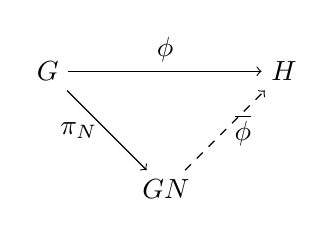
\begin{tikzpicture}
		\node (V) at (0,0) {$G$};
		\node (W) at (3,0) {$H$};
		\node (R) at (1.5,-1.5) {$\lnkset{G}{N}$};
		\draw[->, above] (V) to node {$\phi$} (W);
		\draw[->, left] (V)  to node {$\pi_N$} (R);
		\draw[->, right, dashed] (R)  to node {$\overline{\phi}$} (W);
		\end{tikzpicture}
	\end{center}
\end{proposition}
\begin{proof}
	Existiert so ein $\overline{\phi}$, so ist $\overline{\phi}(gN)=(\overline{\phi}\circ \pi_N)(g)=\phi(g)$ eindeutig bestimmt. Definiere $\overline{\phi}$ nun so.
	\begin{itemize}
		\item $\overline{\phi}$ ist wohldefiniert: $gN = g'N \overset{\propref{1_2_8}}{\Rightarrow}\exists g'=gn$ für ein $n\in N\Rightarrow \phi(g')=\phi(g)\cdot \underbrace{\phi(n)}_{=1}=\phi(g)$, da $n\in\Ker(\phi)$
		\item $\overline{\phi}$ ist Homomorphismus: $\overline{\phi}(gN\cdot g'N) = \overline{\phi}(gg'N)=\phi(gg')=\phi(g)\cdot\phi(g')=\overline{\phi}(gN)\cdot\overline{\phi}(g'N)$
	\end{itemize}
\end{proof}

\begin{conclusion}
	\proplbl{1_3_9}
	Ein Gruppenhomomorphismus $\phi:G\to H$ liefert einen Isomorphismus
	\begin{align}
		\overline{\phi}:\lnkset{G}{\Ker(\phi)}\xrightarrow{\cong}\Image(\phi)\le H\notag
	\end{align}
\end{conclusion}

\begin{conclusion}[1. Homomorphiesatz]
	Seien $H\le G$ und $N\unlhd G$. Der Homomorphismus
	\begin{align}
		\phi: H\overset{i}{\hookrightarrow} HN\xrightarrow{\pi_N}\lnkset{HN}{N}\notag
	\end{align}
	induziert einen Isomorphismus
	\begin{align}
		\overline{\phi}:\lnkset{H}{H\cap N}\xrightarrow{\cong}\lnkset{HN}{N}\notag
	\end{align}
\end{conclusion}
\begin{proof}
	\begin{itemize}
		\item $\phi$ ist surjektiv: Für $h\in H$ und $n\in N$ ist
		\begin{align}
			hnN=hN=\phi(h)\in\phi(H)=\Image(\phi)\notag
		\end{align}
		\item $\Ker(\phi)=H\cap\Ker(\pi_N)=H\cap N$
	\end{itemize}
	Mit \propref{1_3_9} folgt die Behauptung.
\end{proof}

\begin{conclusion}[2. Homomorphiesatz]
	Seien $N\unlhd G$ und $N\le H\unlhd G$. Der Homomorphismus $\pi_H:G\to\lnkset{G}{H}$ induziert einen Isomorphismus
	\begin{align}
		\lnkset{(\lnkset{G}{N})}{(\lnkset{H}{N})}\xrightarrow{\cong}\lnkset{G}{H}\notag
	\end{align}
\end{conclusion}
\begin{proof}
	Da $N\le H$ liefert $\pi_H$ einen Epimorphismus (mit \propref{1_3_8}) $\overline{\pi_H}:\lnkset{G}{N}\to \lnkset{G}{H}$.
	\begin{center}
		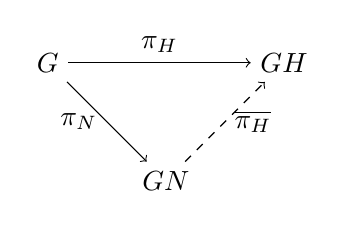
\begin{tikzpicture}
		\node (V) at (0,0) {$G$};
		\node (W) at (3,0) {$\lnkset{G}{H}$};
		\node (R) at (1.5,-1.5) {$\lnkset{G}{N}$};
		\draw[->, above] (V) to node {$\pi_H$} (W);
		\draw[->, left] (V)  to node {$\pi_N$} (R);
		\draw[->, right, dashed] (R)  to node {$\overline{\pi_H}$} (W);
		\end{tikzpicture}
	\end{center}
	Dieser hat Kern $\Ker(\overline{\pi_H})?\lnkset{H}{N}$, induziert nach \propref{1_3_9} einen Isomorphismus
	\begin{align}
		\lnkset{(\lnkset{G}{N})}{\Ker(\overline{\pi_H})}\xrightarrow{\cong}\Image(\overline{\pi_H})=\lnkset{G}{H}\notag
	\end{align}
\end{proof}

\begin{definition}[Konjugation]
	Seien $x,x',g\in G$ und $H,H'\le G$.
	\begin{enumerate}[label=(\alph*)]
		\item $x^g:= g^{-1}xg$, \begriff{Konjugation} von $x$ mit $g$
		\item $x$ und $x'$ sind \begriff{konjugiert} (in $G$)$\Leftrightarrow\exists g\in G$: $x'=x^g$
		\item $H$ und $H'$ heißen \emph{konjugiert} (in $G$)$\Leftrightarrow\exists g\in G$: $H'=H^g=\{h^g\mid h\in H\}$
	\end{enumerate}
\end{definition}

\begin{lemma}
	Die Abbildung
	\begin{align}
		\Int:\begin{cases}
			G\to \Aut(G) \\ g\mapsto (x\mapsto x^g)
		\end{cases}\notag
	\end{align}
	ist ein Gruppenhomomorphismus.
\end{lemma}
\begin{proof}
	\begin{itemize}
		\item $\Int(g)\in\Hom(G,G)$: $(xy)^g=g^{-1}xyg=g^{-1}xgg^{-1}yg=x^g\cdot y^g$
		\item $(x^g)^h=h^{-1}g^{-1}xgh=(gh)^{-1}x(gh)=x^{gh}$
		\item $\Int(g)\in\Aut(G)$: Umkehrabbildung zu $\Int(g)$ ist $\Int(g^{-1})$
		\item $\Int(g)\in\Hom(G,\Aut(G))$:
		\begin{align}
			\Int(gh)=\Int(h)\circ\Int(g)=\Int(g)\cdot\Int(h)\notag
		\end{align}
	\end{itemize}
\end{proof}

\begin{definition}[innere Automorphismen, Zentrum, charakteristische Gruppe]
	\begin{enumerate}[label=(\alph*)]
		\item $\Inn(G)=\Image(\Int)\le\Aut(G)$, die Gruppe der \begriff{inneren Automorphismen} von $G$
		\item $\Z(G)=\Ker(\Int)=\{g\in G\mid xg=gx\quad\forall x\in G\}$, das \begriff{Zentrum} von $G$
		\item $H\le G$ ist \begriff[Gruppe!]{charakteristisch} $\Leftrightarrow\forall\sigma\in\Aut(G)$: $H=H^\sigma$
	\end{enumerate}
\end{definition}

\begin{remark}
	\begin{enumerate}[label=(\alph*)]
		\item Konjugation ist eine Äquivalenzrelation
		\item $H\le G$ ist normal $\Leftrightarrow H=H^\sigma\quad\forall\sigma\in\Inn(G)$
		\item Deshalb gilt für $H\le G$: $H$ ist charakteristisch $\Rightarrow$ $H$ ist normal
	\end{enumerate}
\end{remark}

\begin{example}
	$\Z(G)$ ist charakteristisch in $G$
\end{example}